\chapter{Methodology}
\label{chp:methodology} 
In this thesis the \gls{hls}-tool, LegUp, is investigated to see whether it can be used as a part of framework for hardware architectural exploration. This chapter describes the setup of the tool and gives an introduction to settings and constraints that are needed to build the framework. A sketch and description of a proposed framework is also presented, and the implementation of the reference designs, described in \cref{sec:refdes}, is listed.
\section{LegUp setup}
The developers of LegUp has provided a \gls{vdi}-file for VirtualBox, to let users get started with the tool quickly. The image contains the \gls{os} \textit{Ubuntu 14.04} and comes ready with all the tools needed for running \gls{hls}, including web editions of \textit{ModelSim} for simulation and \textit{Altera Quartus II} for synthesis. The tool can also be installed from source code, which will be necessary if the tool shall be incorporated into an existing work-flow or server infrastructure.
For this thesis, an isolated test-environment were needed and thus, the provided \gls{vdi}-file were appropriate. The image containing \textit{LegUp 4.0} were downloaded from the LegUp web-page and setup in VirtualBox according to the instructions given on the web-page \cite{legupgetstarted}. 

\section{HLS constraints and configuration}
LegUp use \gls{tcl}-files for setting constraints and configuring the \gls{hls}-flow. This section will look on a set of \gls{tcl}-commands that is relevant when creating \gls{hdl}-code compliant with \gls{asic} synthesis and some that can be used for a architectural exploration framework. Other available constraints are described in \cite{legupconst}.
\subsection{\label{subsec:hlsreqconst}Required settings}
The following commands are required in order for LegUp to generate Verilog suitable for synthesis towards an \gls{asic} implementation:
\begin{description}
  \item[VSIM\_NO\_ASSERT] \hfill \\
      When set to 1, this constrain cause assertions to be disabled in the Verilog output used to debug LegUp. This has to be set to remove synthesis errors caused by triple-equality ($===$) assertions. \hfill \\
      \textbf{Required setting:} \textit{1}
  \item[INFERRED\_RAMS] \hfill \\
      Use Verilog to infer RAMs instead of instantiating an Altera altsyncram module. Inferred RAMs don’t support structs (no byte-enable) so enabling this means that the C-program cannot contain structs. \hfill \\
      \textbf{Required setting:} \textit{1}
  \item[INFERRED\_RAM\_FORMAT] \hfill \\
      Ensures that for inferred dual-ported RAMs, the behaviour of both ports of the RAM are defined in the same Verilog \textit{always} block (Altera has ports in separate \textit{always} blocks). Altera format gives error "multiple drivers" when synthesizing.\hfill \\
      \textbf{Required setting:} \textit{xilinx}
  \item[DIVIDER\_MODULE] \hfill \\
      This uses generic divider modules, instead of the Altera primitives.\hfill \\
      \textbf{Required setting:} \textit{generic}
  \item[SDC\_NO\_CHAINING] \hfill \\
      Chaining is a concept in \gls{hls} that allows operators to be stitched together combinationally in a single clock cycle, provided a target clock period constraint is met. When this parameter is set to 1, chaining is disabled and every operator will be scheduled in its own \gls{fsm} state. This will generally increase the number of cycles in the overall schedule (bad), but it may help the circuit Fmax (good). As long as we don't have device characterization (for the \gls{asic} target, this option should be enabled.\hfill \\
      \textbf{Required setting:} \textit{1}
  \item[EXPLICIT\_LPM\_MULTS] \hfill \\
      This parameter explicitly instantiate all multipliers as Altera lpm\_mult modules. When this is off, multiplications are instantiated using the Verilog multiply operator.\hfill \\
      \textbf{Required setting:} \textit{0}
\end{description}
\subsection{Framework settings and constraints:}
The following commands can be used to vary the output from LegUp based on preferred goals like area or speed:
\begin{description}
  \item[set\_resource\_constraint] \hfill \\
      Constrains the number of times a given operation can occur in a cycle. Increasing this parameter can allow instantiating of more modules performing the same operation, at the cost of increased area usage. 
  \item[set\_operation\_sharing] \hfill \\
      Operation sharing adds multiplexing before and after an operation so that it can be used for multiple operations. This saves area by avoiding duplicate hardware, but multiplexers also requires area. Operations requiring less area than the necessary multiplexers, should therefore not be shared.
  \item[ENABLE\_PATTERN\_SHARING] \hfill \\
      Enables resource sharing for patterns of computational operators in a program’s dataflow graph. The idea is that, in a given program, there may be commonly occurring patterns of operators that could be shared in the hardware, by putting multiplexers on the inputs and steering the right data in at the right time (based on the FSM state). This may save area in certain cases. \cite{hadjis2012impact}
  \item[MB\_MINIMIZE\_HW] \hfill \\
      When enabled, the reduced bit-widths analyzed by the bit-width minimization pass will be used in generating the Verilog design. If enabled, bit-width of some signals can be reduced, leading to decreased area.
  \item[LOCAL\_RAMS] \hfill \\
      Turns on alias analysis to determine when an array is only used in one function. These arrays can be placed in a block ram inside that hardware module instead of in global memory. This increases performance because local rams can be accessed in parallel while global memory is limited to two ports.
  \item[loop\_pipeline] \hfill \\
     This parameter enables pipelining for a given loop in the code. Loop pipelining allows a new iteration of the loop to begin before the current one has completed, achieving higher throughput. In a loop nest, only the innermost loop can be pipelined.
\end{description}
\section{Simulation, synthesis and layout}
Simulation is primarily run to verify the correctness of a system. In this thesis, the simulation tool also generates a \gls{vcd} file, showing all value changes in the design. This file is used in the power-estimation tool later in the flow, to get a realistic input of the actual amount of switching happening in the design. Simulation is performed in the tool Questa Advanced Simulator \cite{questasim} using a testbench. Simulation is run using a script, taking a filelist (.fl) file as input, pointing to the \gls{rtl}-design and testbench locations. Synthesis and layout is performed to extract area information for each of the reference designs and to generate a netlist, used in the power-estimation tool. For synthesis and layout towards \gls{asic} architectures, Nordic Semiconductor's tool-flow is used, consisting of \textit{Synopsys Design Compiler} (synthesis) \cite{syndescomp}, \textit{Synopsys IC Compiler} (layout) \cite{syniccomp} and cell libraries describing 180nm technology. A Makefile is used to run the tools. The \gls{rtl} design is read from a filelist and various \gls{tcl} scripts are run for setup, compilation, elaboration and mapping. An additional \gls{tcl} file sets constraints on the synthesis, for instance drive and load constraints, IO timing constraints and clock details.
\section{Tool-flow}
The creation of an automated tool-flow is an important part of building the framework for architectural exploration.  As mentioned in \cref{sec:motivation} it is desirable to create a framework that automatically can generate \gls{rtl}, simulate, synthesize and estimate power consumption from thousands of different architectural variations. Based on the block diagram of a tool-flow shown in \cref{fig:toolflowblock} we'll describe how this can be achieved. 
\begin{figure}[hbpt]
\centering
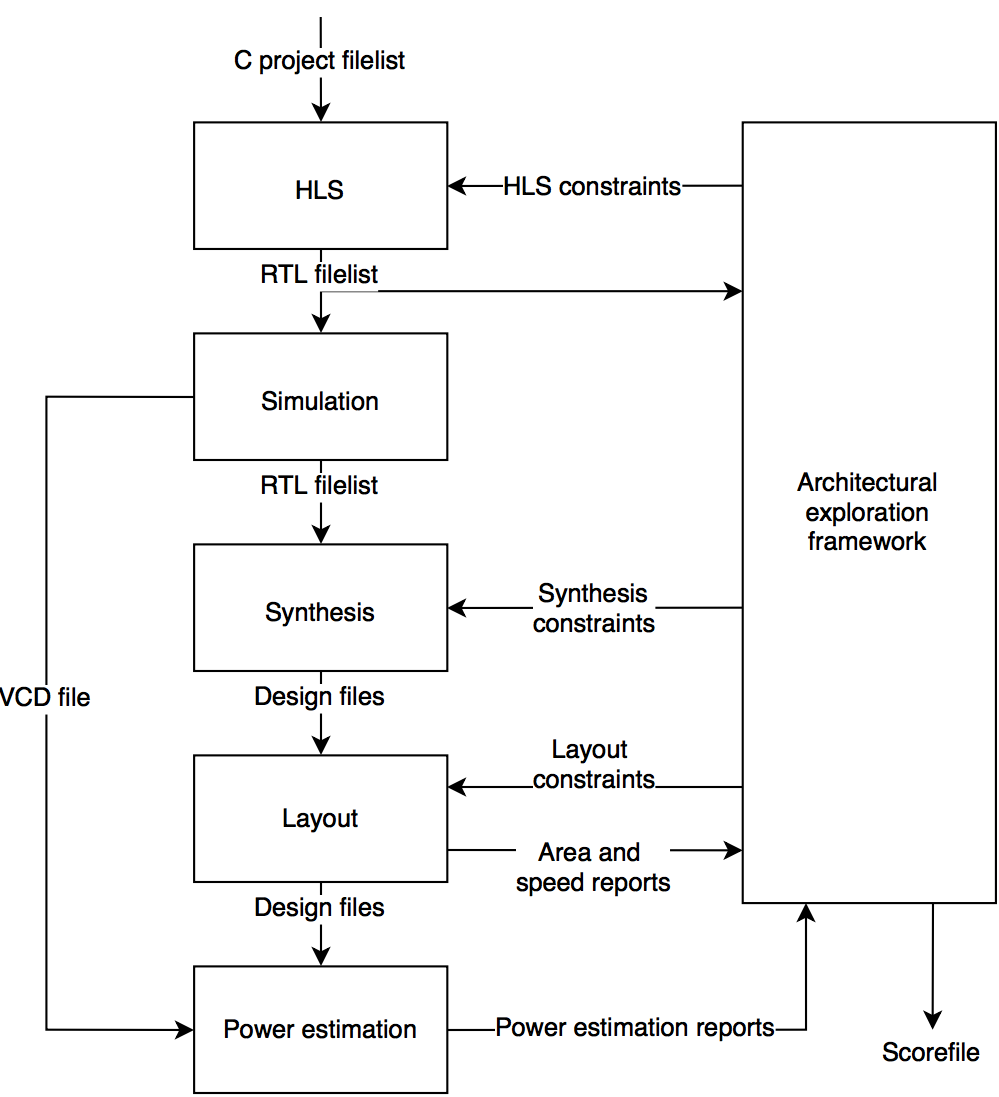
\includegraphics[width=0.6\textwidth]{../figs/Toolflow.png}
\caption{\label{fig:toolflowblock}Block diagram of tool-flow}
\end{figure}
Starting on the right side, a framework is created to control the flow, give constraints to the different steps and keep score of results. On the top of the figure, a filelist pointing to one or multiple C source files is input to the \gls{hls}-tool, in this case, LegUp. Based on the \gls{hls}-constraints given by the framework, LegUp will perform \gls{hls} on the given source files and output a \gls{rtl} filelist pointing to the generated Verilog source files. In the next step, simulation is run on the generated \gls{rtl} to generate a \gls{vcd} file needed for power estimation. It also makes sense to perform simulation in order to verify that the generated design functions properly and as expected. Ideally, the testbench should be generated automatically by the \gls{hls}-tool. LegUp generates a simple testbench, described shortly in \cref{sec:legupoutput}, but this does not include any test-cases. Test-cases needs to be added manually by the designer, but the testbench-shell can be used as a base when creating the testbench. Synthesis and layout are then performed on the \gls{rtl} with respect to constraints given by the framework, generating area and speed reports, as well as post-layout netlist-files describing the final circuitry. In the final step, post-layout netlist files and the \gls{vcd} file from simulation are used to estimate power consumption. The report from power estimation are stored in the framework, together with area and speed results, given constraints and \gls{rtl} filelist. The Framework will run the whole tool-flow multiple times with varying constraints in order to find the best solution. When the tool-flow has been run for all desirable variations, the results will be compared and output in a score-file. This allows the designer to compare different architectural variations and select the best suited solution based on speed, area, and power requirements.

\section{Implementation of reference designs}
In order to compare results of \gls{hls} generated code towards hand-written Verilog, the same reference design are created in both Verilog and C. The source code of each design are listed in \cref{sec:sourcecode}. Due to problems discussed in \cref{sec:encprob}, the designs have not been synthesised. It has therefore not been spent an extensive amount of time on verifying the correctness of the designs.
\subsection{FIR-filter}

The subsections below shows the algorithms and code for implementation of the reference designs.

\subsubsection{Verilog implementation}

A simple implementation of a FIR-filter is listed in \cref{lst:firfilterverilog}. The filter is converted to Verilog from a SystemVerilog example given in \cite{mehler2014digital}. This example is a direct form \gls{fir}-filter of N-order with a data pipeline of N-1. The filter operates on input data, and the output is full precision of internal calculation. Parameters are included in the implementation to easily be able to change the width of the input and the depth of the pipeline.

\lstset{language=SystemVerilog, style=Verilogstyle}
\begin{lstlisting}[caption={FIR-filter implemented in SystemVerilog. Example from \cite{mehler2014digital}},label=lst:firfiltersystemverilog]
module direct2 #(WIDTH = 4, DEPTH = 4)
  (
	input ck, 
	input signed [WIDTH-1:0] dataIn,
	output logic signed[2*WIDTH-1+\$clog2(DEPTH):0] dataOut
	);
	
	logic signed [WIDTH-1:0] sr [DEPTH-2:0];
	logic signed [2*WIDTH-1:0] products [DEPTH-1:0];
	parameter logic signed [WIDTH-1:0] coeff [DEPTH-1:0] = {1,2,3,4};
	logic signed [2*WIDTH-1 + \$clog2(DEPTH):0] sum;
	// Test
	always_ff @(posedge ck) begin
		sr[0] <= dataIn;
		sr[DEPTH-2:1] <= sr[DEPTH-3:0]:
	end
	
	always_comb begin
		products[0] = dataIn * coeff[0];
		for (int i = 1; i < DEPTH; i++)
			products[i] = sr[i-1] * coeff[i];
	end
	
	always_comb begin
		sum = products[0]
		for (int i = 1; i < DEPTH; i++)
			sum = sum + products[i];
	end
	
	always_comb dataOut = sum;
endmodule
\end{lstlisting}
\begin{lstlisting}[caption={FIR-filter implemented in Verilog},label=lst:firfilterverilog]

\end{lstlisting}
\begin{verbatim}
INSERT VERILOG IMPLEMENTATION (OR REFER TO APPENDIX)
\end{verbatim}
\subsubsection{C implementation}
The C implementation of the filter is also based on the SystemVerilog example from \cite{mehler2014digital}, to make the implementations comparable.

\begin{verbatim}
INSERT C-CODE IMPLEMENTATION (OR REFER TO APPENDIX)
\end{verbatim}

\lstset{language=C,style=Cstyle}
\begin{lstlisting}[caption={FIR-filter implemented in C},label=lst:firfilterc]

\end{lstlisting}


\subsection{SAP-1 Architecture}

\subsubsection{Verilog implementation}
The \gls{sap-1} architecture are easily implemented in Verilog. 
\begin{verbatim}
INSERT VERILOG IMPLEMENTATION (OR REFER TO APPENDIX)
\end{verbatim}
\begin{lstlisting}[caption={FIR-filter implemented in C},label=lst:fsap1archverilog]

\end{lstlisting}
\subsubsection{C implementation}
When starting to design the \gls{sap-1} architecture in C, some potential problems were quickly discovered. The first problem is that it is hard to divide the architecture into the modules shown in \cref{fig:sap1arch}. Further, it is hard to force the execution of the program into 6 states, each lasting one clock cycle, when you have no control over the clock. When synthesizing the design into Verilog, it might be reduced to a single \gls{fsm}, doing all the work in just one cycle. The third problem is that as there are no bus capabilities in C, the data are just transferred using standard variables. To get the upper or lower 4 bit of bus, other variables needs to be used. 

\begin{verbatim}
INSERT C-CODE IMPLEMENTATION (OR REFER TO APPENDIX)
\end{verbatim}
\begin{lstlisting}[caption={SAP-1 architecture implemented in C},label=lst:sap1archc]

\end{lstlisting}